%---------------------------------------------------------------------------------------------------
% Einf�hrung
%---------------------------------------------------------------------------------------------------
\newpage
%\part{Anfang}
\pagenumbering{arabic}
\setcounter{page}{1}
\chapter{Einf�hrung}

Bei dem Stichwort \glqq Autonome Systeme\grqq{} f�llt der Gedanke schnell auf Industrie 4.0. Die vierte industrielle Revolution, wie sie von dem Bundesministerium f�r Wirtschaft und Energie genannt wird, beschreibt die selbstorganisierte Produktion durch intelligente und digitale Systeme. \cite{bmwi} Ein solches autonomes System soll als Produktionsstra�e im Verbundprojekt der Hochschule f�r Angewandte Wissenschaft Hamburg mit Hilfe von Transportrobotern, sogenannten Robotinos, realisiert werden.

Zur Realisierung dieser Produktionsstra�e werden bereits zu Beginn der Projektarbeit alle notwendigen Hardwarekomponenten zur Verf�gung gestellt. Zu diesen Hardwarekomponenten geh�ren die Robotinos. Ein Robotino ist ein mobiles Robotersystem mit omnidirektionalem Antrieb, der es dem Roboter erm�glicht zu jeder Zeit in jede beliebige Richtung fahren zu k�nnen. Sie werden mittels ArUco-Marker und Deckenkameras lokalisiert. Bei den zu transportierenden Werkst�cken handelt es sich um runde Bausteine. Diese Bausteine sind mit einem RFID-Transponder ausgestattet und k�nnen von den Leseger�ten an den Stationen gelesen werden. Insgesamt gibt es vier Stationen, die beidseitig angefahren werden k�nnen. Diese Stationen repr�sentieren die Lager bzw. Maschinen, zu denen die Werkst�cke, je nach Auftrag, transportiert werden m�ssen. Zwei zus�tzliche Stationen sind als Ladestationen f�r die Robotinos ausgelegt.

Auf Grund der Komplexit�t dieses Projektes, wird das Gesamtprojekt in einzelne Aufgabenpakete unterteilt, welche in Gruppenarbeit von drei bis vier Personen zu bearbeiten sind. Insgesamt gibt es f�nf Gewerke, darunter die Auftragskoordination, Bahnplanung  und Regelung, deren Ziel es ist ein funktionsf�higes und zuverl�ssiges Gesamtsystem zu entwickeln. Zus�tzlich wird sich zum Ziel gesetzt, eine neue Version des Robotinos, den Robotino 2.0, am Ablauf der Produktionsstra�e zu beteiligen.

Um dieses Gesamtziel zu erreichen, sind gemeinsame Schnittstellen, stetige Kommunikation, sowie abgestimmtes Zeitmanagement von gro�er Bedeutung. 

In der vorliegenden Dokumentation wird die Umsetzung der Bahnplanung eingehend erl�utert. Zu den Aufgabenbereichen der Bahnplanung geh�rt die Vorgabe eines Weges f�r den Robotino von einem Start- zu einem Zielpunkt, sowie die Kollisionsvermeidung mit statischen und dynamischen Hindernissen. 
\newpage

\chapter{Aufgabenstellung}

Aufgabe der Bahnplanung ist es, den Robotino von einer beliebigen Startposition im bekannten Raum zu einem vorgegebenen Ziel fahren zu lassen. Dabei ist zu beachten, dass es zu keiner Zeit zu einer Kollision mit dynamischen oder statischen Hindernissen kommt. 

F�r die Aufnahme und Abgabe der Werkst�cke, also das Werkst�ckhandling allgemein, muss sowohl zu der Auftragskoordination, wie auch zu der Regelung eine geeignete und zuverl�ssige Schnittstelle generiert werden. 
Dazu geh�rt auch das Anfahren an die Stationen und das Fehler-Handling. 

Die Algorithmen zur Realisierung der Bahnplanung und Kollisionsvermeidung sind in Matlab/Simulink zu implementieren. Der interne Programmablauf ist als Simulink/Stateflow mittels Blockschaltbilder zu realisieren.
Die zu erstellende Software wird auf jeden einzelnen Robotino geladen und l�uft dort dezentral als xPC-Target.
\newpage

\chapter{Bahnplanung}

Die Navigation, also das effiziente und kollisionsfreie Bewegen im Raum, geh�rt zu den Hauptaufgaben von autonomen mobilen Robotern. Um zum Beispiel Produktionsstra�en zukunftsf�hig und effizienter zu gestalten, m�ssen die Robotinos konkreten Aufgaben wie \glqq Fahre zum Zielpunkt XY und nehme das Werkst�ck auf\grqq{} �bernehmen und abarbeiten k�nnen. Dazu muss der Robotino zu jeder Zeit folgende Fragen beantworten k�nnen: \glqq Wo befinde ich mich? Wo muss ich hin? Wie gelange ich dort hin?\grqq \cite{WegPlanung}

Anhand dieser Fragen l�sst sich die Bahnplanung in drei Bereiche unterteilen:
\begin{itemize}
\item \textbf{Lokalisierung:} Genau Positionsbestimmung des Robotinos im bekannten Raum
\item \textbf{Kartenerstellung:} Vom Roboter �ber Sensordaten erstellte oder durch Softwareimplementierung bekannte Karte des Raumes
\item \textbf{Trajektoriengenerierung:} Berechnung von Trajektorien vom Startpunkt zum Ziel
\end{itemize}
\section{Lokalisierung}
Eine Bahnplanung kann nur dann erfolgen, wenn der Roboter seine eigene Position zu jeder Zeit lokalisieren kann. 
In dem Fall des hier ausgearbeiteten Projektes erfolgt die Lokalisierung �ber Deckenkameras, die mittels UDP-Kommunikation den Robotinos ihre eigene Position, aber auch die der anderen Robotinos im bekannten Raum senden. Intern wird �ber den Raum ein Koordinatensystem gelegt,so dass die genaue Position der Roboter in x- und y-Richtung ausgegeben werden kann. Zu diesem Zweck sind die Robotinos mit ArUco-Markern ausgestattet. Um ein zuverl�ssiges Gesamtsystem zu erschaffen und die Ausfallwahrscheinlichkeit zu minimieren, erfolgt die Lokalisierung zus�tzlich �ber Positionsdaten des Gewerks 3 \glqq Regelung\grqq. Somit wird sichergestellt, dass bei ungenauen oder nicht vorhandenen Kameradaten die Robotinoposition zu jeder Zeit bekannt und ein unterbrechungsfreier Ablauf des Prozesses gegeben ist. \cite{WegPlanung}
\section{Kartenerstellung}
Mit bekannten Karten und vom Roboter durch die Sensorik erstellte Karten helfen beim Wegfinden. Durch eine vorab erstellte Karte k�nnen Hindernisse und Sackgassen implementiert werden, die von dem Transportroboter gemieden werden m�ssen. Kennt der Robotino seine Umgebung durch eine Karte kann �ber Selbstlokalisierung ein optimaler Pfad generiert werden.\cite{WegPlanung} Im Fall des vorliegenden Projektes muss der Roboter nicht durch willk�rliches Fahren im Raum vorab eine Karte von unbefahrbaren Punkten sammeln. Den Robotinos sind die festen Hindernisse, das hei�t Lager, Lade- und Werkstationen, auf Grund der implementierten Programmierung von vornherein bekannt.
\section{Trajektoriengenergierung}
Durch die Bahnplanung k�nnen kollisionsfreie Trajektorien von einem Start- zu einem Zielpunkt generiert werden. Als Trajektorie wird in der Physik der Bewegungsverlauf des Roboters als Kurve im Raum bezeichnet, also die Zustands�nderung relativ zum Koordinatensystem �ber die Zeit. Es werden Solltrajektorien berechnet, die dem Gewerk 3 \glqq Regelung\grqq{} �ber eine definierte Schnittstelle �bergeben werden. �ber diese Trajektorie wird der Robotino zum Ziel gef�hrt.

Die Literatur bietet viele verschiedene Ans�tze zur Berechnung des bestm�glichen Pfades. Die Auswahl eines solchen Ansatzes h�ngt von der projektspezifischen Aufgabenstellung und Definition von \glqq bester Pfad\grqq{} ab. \glqq Bester Weg\grqq{} wird im Allgemeinen mit k�rzester Distanz assoziiert. Es kann aber auch andere Faktoren beinhalten, die angeben wie \glqq teuer\grqq{} ein Weg ist. Ist der Untergrund zum Beispiel schlecht befahrbar, so k�nnte es schneller sein einen Umweg zu fahren. Auch k�nnten kinematische und dynamische Eigenschaften des Roboters in die Definition mit eingehen, so dass Pfade vermieden werden, die Kurven beinhalten, die der Roboter nicht fahren kann. Auch Kriterien wie Energieeffizienz, Schnelligkeit und gr��tm�glicher Abstand zu Hindernissen haben je nach Aufgabenstellung eine andere Gewichtung bez�glich des Bahnplanungsansatzes. Allgemein wird in der Bahnplanung zwischen globaler und lokaler Bahnplanung unterschieden. 

Im Nachfolgenden werden unterschiedliche Bahnplanungsans�tze betrachtet und bewertet.
\subsection{Globale Bahnplanung}
Bei der globalen Bahnplanung, in der englischsprachigen Literatur auch bekannt als \glqq Map-Based Planing\grqq{} m�ssen dem Robotino der Raum und die sich darin befindlichen statischen Hindernisse und Sackgassen vollst�ndig bekannt sein, um diese in jedem Fall zu vermeiden. Im Folgenden werden zwei M�glichkeiten der globalen Bahnplanung beschrieben: 
\begin{itemize}
\item \textbf{Sichtbarkeitsgraph-Methode mit A*-Algorithmus}
\item \textbf{Occupancy Grid mit D*-Algorithmus}
\end{itemize}

\subsubsection{Sichtbarbeitsgraph Methode mit A*}
Der Sichtbarkeitsgraph (engl. Visible graphs) ist eine Methode um den k�rzesten Pfad zwischen zwei Punkten zu finden. 
Diese Methode setzt voraus, dass vorab Start- und Zielpunkt, so wie Eckpunkte der statischen Hindernisse klar definiert und bekannt sind.  
Die Eckpunkte der Hindernisse werden dann durch eine Kante verbunden, wenn eine gerade Verbindungslinie gezogen werden kann, ohne andere Hindernisse zu schneiden. Dadurch werden Eckpunkte zu Knotenpunkten. Die Hindernisse mit den Verbindungslinien ist in Abbildung \ref{fig:Sichtbarkeitsgraph} dargestellt. \cite{WegPlanung}

\begin{figure}[h]
	\centering	
	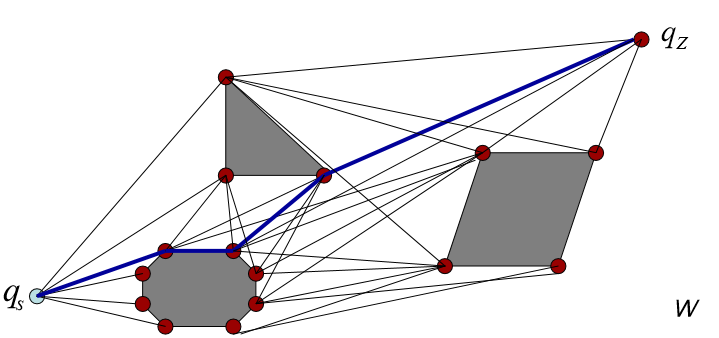
\includegraphics[width=12cm]{BilderInke/Sichtbarkeitsgraph.png}
	\caption{Beispiel Sichtbarkeitsgraph, Graue Felder sind Hindernisse, blaue Linie ist optimaler Pfad}
	\label{fig:Sichtbarkeitsgraph}
	\cite{WegPlanung}
\end{figure}

Durch Einsatz der A*-Methode kann so der optimale Pfad bestimmt werden. Die Kanten zwischen zwei Knotenpunkten werden von dem Algorithmus je nach Anforderung, beispielsweise k�rzester Weg, gewichtet. Je gr��er diese Gewichtung ist, desto weiter Weg befindet sich der Knotenpunkt am anderen Ende der Kante. Die direkte Entfernung eines Knotenpunktes zum Zielpunkt wird gesch�tzt, so dass die Knoten ebenfalls eine Gewichtung bekommen. 

Vom Zielpunkt aus werden nun alle Knoten betrachtet, die �ber eine Kante erreicht werden k�nnen. Der aus der Betrachtung hervorgehende Knotenpunkt, der die geringste direkte Entfernung zum Ziel aufweist, wird als n�chstes untersucht. Die anderen werden gespeichert und im weiteren Verlauf mit Konten hinsichtlich ihrer Gewichtung verglichen. Punkte, die bereits betrachtet wurden, werden  als \glqq untersucht \grqq{} markiert. Dieses Verfahren wiederholt sich so lange bis der optimale Pfad gefunden wurde. Ein solcher Pfad ist in der obenstehenden Abbildung als dicke blaue Linie dargestellt. 

Ein Vorteil dieser Methode ist, dass immer der optimale Pfad vom Start zum Ziel gefunden wird. Nachteile sind jedoch, dass der Pfad immer direkt an den Ecken und Kanten der Hindernisse entlang f�hrt. Au�erdem kann bei vielen Hindernissen, beispielsweise Hindernisse mit vielen Ecken und Kanten, ein sehr gro�er Graph entstehen, der viel Rechenzeit in Anspruch nimmt. 

\subsubsection{Occupancy Grid mit D*-Algorithmus}
Wie der Name \glqq Occupancy Grid\grqq{} vermuten l�sst, wird der Raum in ein Gitternetz unterteilt. Jede entstehende Zelle kann mit einer \glqq 1\grqq{} f�r \glqq belegt\grqq{} und \glqq 0\grqq{} f�r \glqq frei\grqq{} versehen werden. Dadurch entsteht eine Umgebungskarte, in der Hindernisse und freier Raum zum Fahren klar definiert sind. In der Abbildung \ref{fig:OccupancyGrid} ist ein Beispiel des Occupancy Grids dargestellt. Dabei sind anstatt Zahlen in den Zellen die freien Bereiche wei� und die besetzten Bereiche rot dargestellt. Der �bersichtlichkeit halber ist ein gr��eres Gitternetz dargestellt, als eigentlich unterteilt.\cite{Robotics}\\

\begin{figure}[H]
	\centering	
	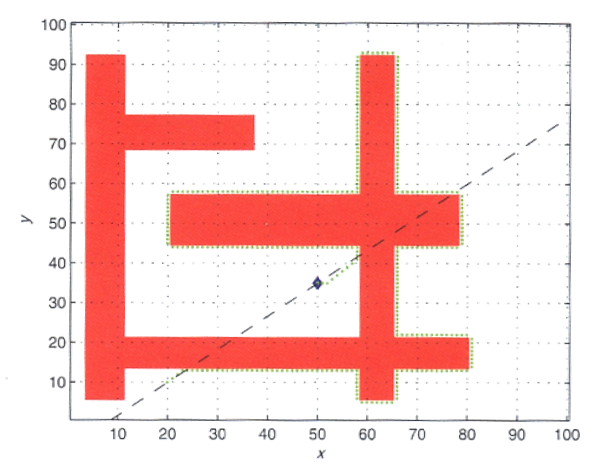
\includegraphics[width=10cm]{BilderInke/OccupancyGrid.png}
	\caption{Beispiel Occupancy Grid, Rot-Hindernisse, Wei�-befahrbarer Raum}
	\label{fig:OccupancyGrid}
	\cite{Robotics}
\end{figure}

Der D*-Algorithmus ver�ndert die Bewertung der einzelnen Zellen mit einem neuen Wert, der die \glqq Kosten\grqq der Zelle repr�sentiert. Zellen, die zu einem Hindernis geh�ren werden mit \glqq $ \infty $\grqq gewichtet. Je h�her die Gewichtung ist, desto weiter weg befindet sich das Ziel. Mit diesem Algorithmus wird immer der optimale Pfad gefunden. Je nach Aufgabenstellung kann diese Gewichtung zum Beispiel Distanz oder Zeit bedeuten. 
In der nachstehenden Abbildung \ref{fig:Occupancy Grid mit D*-Algorithmus} ist der geplante Weg von dem Startpunkt zum Ziel mittels gr�n gepunkteter Linie dargestellt. Die Hindernisse sind rot markiert. Die Intensit�t des Grautons im Hintergrund gibt in diesem Fall die Entfernung zum Ziel an. 
\begin{figure}[H]
	\centering	
	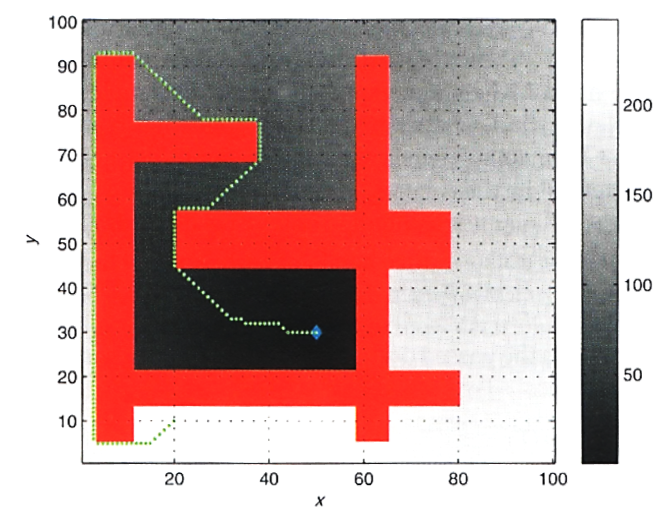
\includegraphics[width=10cm]{BilderInke/DStern.png}
	\caption{Beispiel Occupancy Grid mit D*, Rot-Hindernisse, Intensit�t des Graus im Hintergrunds repr�sentiert die Entfernung zum Ziel; blauer Punkt entspricht Ziel}
	\label{fig:Occupancy Grid mit D*-Algorithmus}
	\cite{Robotics}
\end{figure}

Ein Vorteil dieser Methode ist, dass der Weg schrittweise neu geplant werden kann. Sollte der Raum anders sein, als zuvor in dem Gitternetz eingetragen, eine Zelle beispielsweise teurer sein als geplant, so kann stufenweise ein besserer Pfad gefunden werden. Die Berechnung des neuen Weges erfordert nicht so viel Rechenleistung, wie eine komplett neue Wegplanung, da nur die Zellen in direkter Umgebung betrachtet werden. Die Anfangsberechnung ist hingegen sehr rechenintensiv. Zudem ben�tigt das Occupancy Grid bei hoher Aufl�sung viel Speicherplatz.

\subsection{Lokale Bahnplanung}
Die lokale Bahnplanung betrachtet nur das direkte Umfeld des Roboters. Lokale Bahnplanungsalgorithmen planen den Weg zum Ziel weniger vorausschauend. Daher ben�tigen sie in der Regel weniger Rechenzeit und sind somit schneller als globale Bahnplanungsmethoden. Mit den aktuellen Umgebungsdaten und Sensorinformationen wird ein lokales Navigationsziel angestrebt. Ziel ist hierbei die reaktive Kollisionsvermeidung. 
Im Folgenden werden zwei M�glichkeiten den lokalen Bahnplanung beschrieben: 
\begin{itemize}
\item \textbf{Bug-Algorithmus}
\item \textbf{Potentialfeld-Methode}
\end{itemize}

\subsubsection{Bug-Algorithmus}
Der \glqq Bug-Algorithmus \grqq{} ist im Allgemeinen eine reaktive Navigationsmethode und basiert auf dem Prinzip, dass sich der Roboter so lange entlang eines Hindernisses bewegt, bis er wieder freie Fahrt in Richtung Ziel hat. Es gibt verschiedene Algorithmen, die diese Methode verfolgen. Dazu geh�rt der \glqq Bug1 -\grqq, \glqq Bug2-\grqq, \glqq Bug3-\grqq und \glqq DistBug-Algorithmus \grqq{}. Im Folgenden wird nur der Bug2-Algorithmus n�hergehend erl�utert. \cite{Bug2} \cite{WegPlanung} 

Unter Verwendung des betrachteten Algorithmus kennt der Roboter zu jeder Zeit den direkten Weg zwischen seiner Startposition und dem Ziel. Hierbei werden m�gliche Hindernisse zun�chst nicht ber�cksichtigt. Abgesehen von einem Ziel im globalen Raum, kennt der Roboter nur seine direkte Umgebung. Der direkte Weg wird hier m-Linie genannt. Ein Beispiel ist in der untenstehenden Abbildung \ref{fig:Bug2_m-Linie} dargestellt.

\begin{figure}[H]
	\centering	
	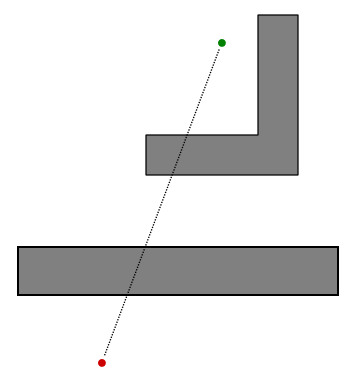
\includegraphics[width=5cm]{BilderInke/Bug2_m-Linie.png}
	\caption{Bu2-Algorithmus, Grauen Fl�chen: Hindernisse, Roter Punkt: Startpunkt, Gr�ner Punkt: Ziel, Verbindungslinie: m-Linie}
	\label{fig:Bug2_m-Linie}
	\cite{Bug2}
\end{figure}
Der rote Punkt in der Abbildung ist die Startposition und der gr�ne das Ziel. 
Die Anweisung des Algorithmus an den Roboter k�nnen in drei einfache Befehle unterteilt werden. 

\begin{itemize}
\item \textsl{Fahre auf der m-Linie Richtung Ziel}
\item \textsl{Ist ein Hindernis im Weg, dann fahre an dessen Kante entlang, bis die  m-Linie wieder erreicht wird}
\item \textsl{Ist die m-Linie wieder erreicht, verlasse das Hindernis und fahre weiter Richtung Ziel}
\end{itemize}

Wie ein m�glicher Weg des Roboters unter dem Bug2-Algorithmus aussehen k�nnte, ist in Abbildung \ref{fig:Bug2} zusehen. Die orangene Linie zeigt dabei den Fahrweg des Roboters

\begin{figure}[H]
	\centering	
	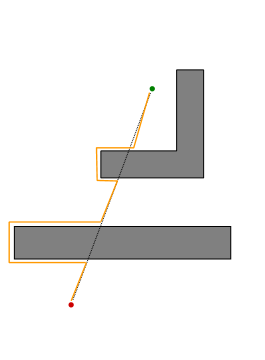
\includegraphics[width=5cm]{BilderInke/Bug2.png}
	\caption{Bu2-Algorithmus, Fahrweg des Roboters ist in orange dargestellt}
	\label{fig:Bug2}
	\cite{Bug2}
\end{figure}

Der Bug2-Algorithmus ist ein vergleichsweise einfacher Algorithmus. Das Entlangfahren an den Hindernissen kann nur in eine Richtung, links oder rechts, vorgegeben werden. Somit ist nicht garantiert, dass immer der optimale Pfad gefunden wird. Au�erdem kann es zu einer Art \glqq Deadlock\grqq{} kommen, wenn der Roboter an einer Kante des Hindernissen entlang fahren muss, die m-Linie jedoch nicht wieder findet. Ein solches Szenario ist in Abbildung \ref{fig:Bug2_Problem} dargestellt. 

\begin{figure}[H]
	\centering	
	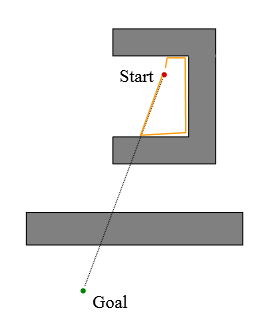
\includegraphics[width=5cm]{BilderInke/Bug2_Problem.png}
	\caption{Bu2-Algorithmus, m�glicher Deadlock,  Fahrweg des Roboters ist in orange dargestellt}
	\label{fig:Bug2_Problem}
	\cite{Bug2}
\end{figure}

\subsubsection{Potentialfeld-Methode}
Bei der Potentailfeld-Methode ist der Roboter k�nstlichen Kr�ften von Zielen und Hindernissen ausgesetzt. Die hohen Potentiale sto�en den Roboter ab, niedrigere Potentiale ziehen ihn an. Jeder Punkt in dem Konfigurationsraum erh�lt ein Potential. So wird dem Start ein hohes und dem Ziel ein sehr niedriges Potential zugeordnet. Hindernisse bekommen sehr hohe Potentiale. Die Bewegungsrichtung des Roboters kann �ber die Gradientenberechnung des Potentialfeldes erfolgen, da der Roboter auf seinem Weg vom Start zum Ziel dem negativen Gradienten des globalen Potentialfeldes folgt. In die Berechnung des Gradienten gehen nur die Hindernisse mit ein, die sich in relativer N�he zum Roboter befinden.\cite{WegPlanung} In der Abbildung \ref{fig:Potentialfeld} ist ein Beispiel eines Potentialfeldes dargestellt. Das niedrige Potential des Ziels ist in blau dargestellt. 

\begin{figure}[H]
	\centering	
	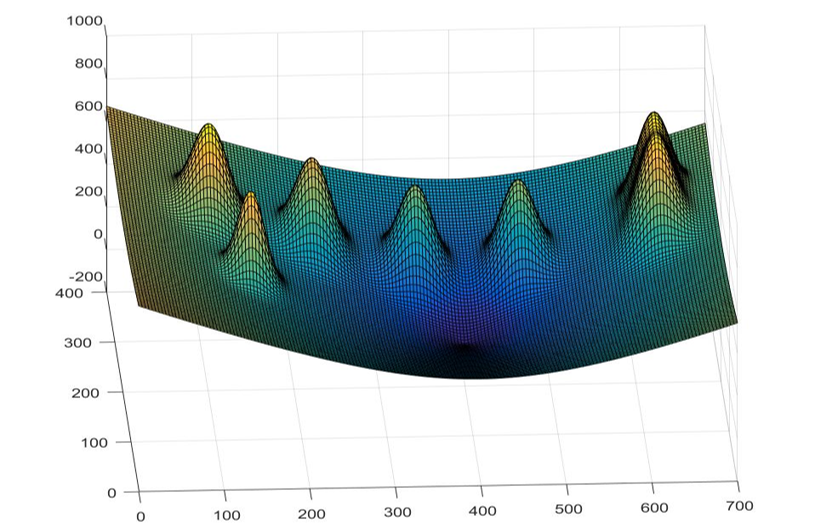
\includegraphics[width=15cm]{BilderInke/Potentialfeld.png}
	\caption{Beispiel Potentialfeld}
	\label{fig:Potentialfeld}
\end{figure}

Die Vorteile der Potentialfeld-Methode sind sowohl die einfache Implementierung als auch die geringe Rechenzeit. Durch die Echtzeit-Kollisionsvermeidung ist das System sehr dynamisch. Es besteht jedoch die Gefahr, dass lokale Minima entstehen, aus denen der Robotino nicht wieder raus kommt.  

\section{Ausgew�hltes Konzept}

An der zu simulierenden Produktionsstra�e sind bis zu f�nf Robotinos gleichzeitig beteiligt. Um einen zuverl�ssigen Produktionsablauf sicherstellen zu k�nnen, werden hohe Anforderungen an die Bahnplanungsmethode gestellt. Die Methode muss dynamisch und zuverl�ssig sein und sollte geringen Rechenaufwand ben�tigen. Die soeben erl�uterten Methoden sind in der Tabelle \ref{tab: Methodenvergleich}, reduziert auf die wichtigsten Eigenschaften, �bersichtliche dargestellt. 

\begin{table}[H]
\caption{Bahnplanungsmethoden nach ihrer Dynamik, Sicherheit, Rechenzeit und Zuverl�ssigkeit bewertet}
 \begin{tabular}{lcccc}
 
  Methode & Dynamik & Sicherheit & Rechenzeit & Zuverl�ssigkeit \\
  \hline 
  Sichtbarkeitsgraph mit A* & gering & mittel & mittel/hoch & sehr hoch \\
  Occupancy Grid mit D* & mittel & hoch & mittel/hoch & hoch \\
  Bug-Methode & mittel & gering & gering & gering \\
  Potentialfeld-Methode & sehr hoch & mittel & gering & hoch \\
  
  \label{tab: Methodenvergleich}
  
 \end{tabular}
\end{table}
Bei sehr hoher Dynamik und hoher Zuverl�ssigkeit ben�tigt die Potentialfeld-Methode nur wenig Rechenzeit. Damit ist sie von den betrachteten Methoden die beste. Das Potentialfeld hat zudem den Vorteil, dass ein komplett autonomes Gesamtsystem geschaffen werden kann, da es f�r die Trajektorienberechnung nicht notwendig ist das Ziel und die Fahrtroute der anderen Robotinos zu kennen. 

\subsection{Gesamtkonzept}

Im Folgenden wird das Gesamtkonzept mit der Bahnplanungsmethode Potentialfeld kurz erl�utert. Genauere Erkl�rungen mit Ausz�gen aus dem Originalprogramm werden anschlie�end erl�utert. 
\begin{figure}[H]
	\centering	
	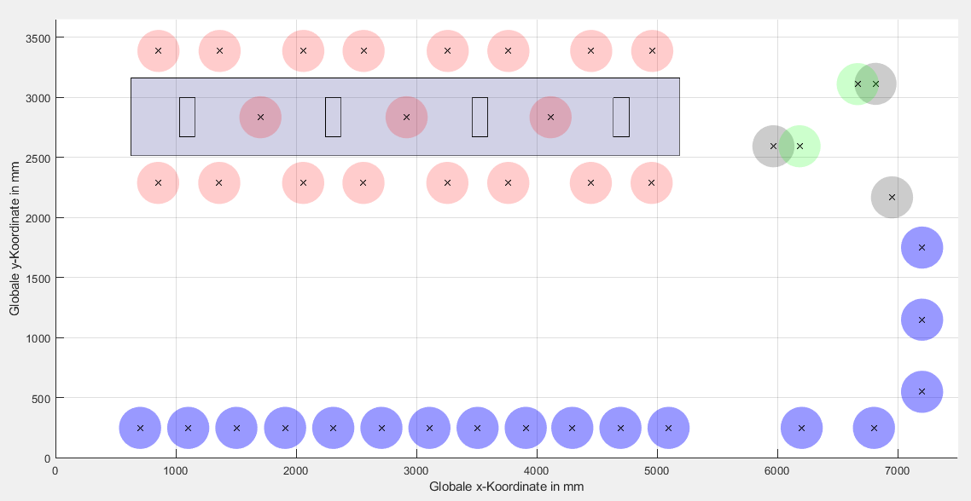
\includegraphics[width=14cm]{BilderInke/KonfigRaum.png}
	\caption{Konfigurationsraum mit Wartepositionen, Fifo-Positionen, Stationen und �bergabepunkten}
	\label{fig:Konfigurationsraum}
\end{figure}
Der Konfigurationsraum ist in Abbildung \ref{fig:Konfigurationsraum} mit globalem Koordinatensystem, eingezeichneten Stationen, Wartepositionen und �bergabepunkten dargestellt. 

\subsubsection{Wartepositionen}
\label{Wartepositionen}
Jedem Robotino wird eine eigene Warteposition am Rand des Konfigurationsraumes zugeordnet. Diese Warteposition ist zu Beginn des Gesamtsystem die Startposition des jeweiligen Robotinos und immer dann Zielposition, wenn der Robotino keinen Auftrag empf�ngt. Sollten alle \glqq Fifo-Pl�tz\grqq{} (vgl. Kapitel \ref{Warteschlange}) einer Station belegt sein, so dass sich ein Robotino nicht mehr anstellen kann, muss er auf seiner Warteposition auf einen freien Platz warten. 

\subsubsection{Stationen und �bergabepunkte}
\label{Stationen und �bergabepunkte}
Wie in Abbildung \ref{fig:Konfigurationsraum} zu sehen ist, befindet sich vor und hinter jeder Station �bergabepunkte. Hat ein Robotino die Aufgabe zu einer Station zu fahren, f�hrt er stattdessen nur vor die Station auf den �bergabepunkt. Ab da wird die Steuerung des Roboters an das Gewerk3 \glqq Regelung\grqq{} �bergeben. Sollten mehrere Robotinos die gleiche Station anfahren wollen, so darf der Robotino die Station zuerst befahren, der den �bergabepunkt zuerst erreicht hat. �ber die �bergabepunkte wird die Station auch wieder verlassen. Der vordere �bergabepunkt wird immer dann genutzt, wenn sich kein weitere Robotino im Fifo befindet. �ber den hinteren �bergabepunkt wird die Station verlassen, wenn ein andere Robotino bereits im Fifo (vgl. Kapitel \ref{Warteschlange}) wartet. 
Das Potentialfeld ist in den Stationen, solange Gewerk3 \glqq Regelung\grqq{} den Robotino steuert, nicht aktiv. Aktiviert beziehungsweise ausgeschaltet wird das Potentialfeld zum Zeitpunkt der �bergabe. Sollte ein Robotino, aufgrund eines notwendigen Ausweichman�vers, in eine Station gedr�ckt werden, so verl�sst er sie unverz�glich nach hinten raus. In diesem Fall bleibt das Potentialfeld aktiv. 

\subsubsection{Warteschlange \glqq Fifo\grqq}
\label{Warteschlange}
Ist eine Station, in die ein Robotino fahren soll, bereits belegt, so f�hrt er zu der zugeh�rigen Warteschlange, dem sogenannten \glqq Fifos\grqq{}. Die Fifos, die sich am Rand des Konfigurationsraumes befinden, sind Wartepositionen f�r die Stationen, um w�hrend des Wartens den befahrbaren Raum nicht zu blockieren. Der Robotino, der die Warteschlange zuerst betreten hat, darf diese, sobald die Station wieder frei ist, auch als erster wieder verlassen. Erst, wenn dieser die Station erreicht hat, r�cken eventuell wartende Robotinos im gleichen Fifo auf. 

\subsubsection{Ladestation}
\label{Ladestation}
Die Ladestationen befinden sich an der rechten Seite des Konfigurationsraumes. Eine Ladestation ist f�r die Robotinos 1.0 und eine weitere f�r den Robotino 2.0. Auch hier sind �bergabepunkte definiert. Aus platztechnischen Gr�nden muss der Robotino 2.0 von hinten an die Ladestation fahren. Um dieses m�glichst effizient zu realisieren, ist der �bergabepunkt f�r diese Ladestation vergleichsweise weit im eigentlichen Transportbereich. Ab diesem Punkt wird an Gewerk3 �bergeben, welches den Robotino 2.0 mittels hoch genauer Regelung vor und in die Ladestation fahren l�sst. 

\subsubsection{Potentialfeld}
\label{Potentialfeld}
Hindernisse im Potentialfeld werden mit hohen Potentialen versehen. Zu diesen Hindernissen geh�ren hier die Stationen und die Robotinos. In Abbildung \ref{fig:Potentialfeld-Fertig} ist das gesamte Potentialfeld dargestellt, das auf jeden Robotino geladen wird. 
\begin{figure}[h!]
	\centering	
	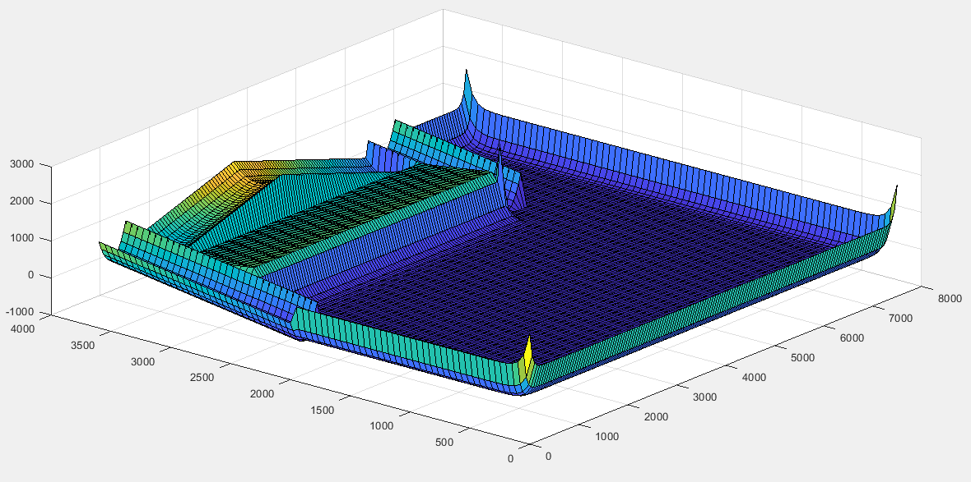
\includegraphics[width=15cm]{BilderInke/Potentialfeld_Fertig.png}
	\caption{Potentialfeld des Konfigurationsraumes eingez�unt in hohe Potentiale zur eindeutigen Begrenzung des Raumes, Stationen als ein hohes Potential dargestellt, Rampen und Fahrrinnen zum leiten der Robotinos, }
	\label{fig:Potentialfeld-Fertig}
\end{figure}

�ber eine Begrenzung durch hohes Potential wird der Raum, in dem sich die Robotinos bewegen d�rfen, eindeutig definiert. Die Stationen sind als ein gesamter Block mit hohem Potential dargestellt, da der Robotino zu keiner Zeit zwischen oder an eine Station fahren soll, wenn nicht zuvor die �bergabe an Gewerk3 erfolgt ist. 
Zur Vermeidung von kritischen Situationen oder lokalen Minima zwischen Stationen und Wand sind Rampen und Fahrrinnen implementiert, die je nach Station den Roboter nach links oder rechts in eine Fahrrinne und von dort in den frei befahrbaren Raum f�hren. 

%\chapter{Konzept}
%\section{Potentialfeld zur Bahngenerierung und Kollisionsvermeidung}
%\subsection{Roboter Umwelt}
%\subsection{Robotino}
%\subsection{Ziel}
%\section{Kollisionsvermeidung durch *ich kann nicht lesen was davor steht* Bereiche}
%\subsection{Selbstorganisation durch Wartebereiche}
%\subsection{Bekannte Hindernisse}
%\subsection{Unbekannte Hindernisse}
%\section{Schnittstellen}
%\subsection{Bahnregelung}
%\subsection{Fertigungsplanung}
%\subsection{Positionsdaten}
%\section{Gesamtprogrammablauf}
%\chapter{Simulation und Testplanung}
%\chapter{Implementierung und Zielsysteme}
%\chapter{Robotino 2.0}
\chapter{Validierung}
%\chapter{Ausblick}
%\chapter{Fazit}






